\section{Multi-Seed Robustness Analysis}
\label{sec:multi_seed_robustness}

This section evaluates the stability of the Gen-MOR models across multiple random seeds. Since neural generative models are stochastic, a single run may not provide a reliable picture of model performance. Multi-seed evaluation helps determine whether reconstruction, classification, and dominance validity are consistent across independent runs.

\subsection{Motivation for Multi-Seed Evaluation}
\label{subsec:motivation_multiseed}

The AE, VAE, and CVAE models can be affected by random initialization, mini-batch ordering, train-validation-test splitting, latent sampling, and dataset generation. For VAE and CVAE models, generation also depends on random samples drawn from the latent prior. These sources of variation can change both standard metrics and DVR.

For this reason, the experiment is repeated over the seed set $\mathcal{R}$ defined in Eq.~\eqref{eq:random_seed_set}. In the current experiment,
\begin{equation}
    \mathcal{R} = \{42, 123, 456, 789, 2024\}.
    \label{eq:actual_multiseed_set}
\end{equation}
For each seed, the same training, evaluation, generation, and dominance verification pipeline is executed. The final results are reported using the mean and standard deviation defined in Eq.~\eqref{eq:metric_mean} and Eq.~\eqref{eq:metric_std}.

\subsection{Reconstruction Stability}
\label{subsec:reconstruction_stability}

Reconstruction stability is evaluated by comparing MSE across seeds. A stable model should have both low average MSE and low standard deviation. Table~\ref{tab:mse_multiseed} reports the multi-seed reconstruction results.

\begin{table}[H]
\centering
\caption{Multi-seed reconstruction stability measured by MSE.}
\label{tab:mse_multiseed}
\begin{tabular}{|l|c|c|}
\hline
\textbf{Model} & \textbf{Mean MSE} & \textbf{Std. Dev.} \\
\hline
AE & $0.0277$ & $0.0061$ \\
VAE & $0.0579$ & $0.0185$ \\
CVAE & $0.0670$ & $0.0242$ \\
\hline
\end{tabular}
\end{table}

The AE has the lowest average reconstruction error and the smallest reconstruction variance. This indicates that the deterministic autoencoder is the most stable model for reconstructing objective-vector plans. The VAE and CVAE have higher mean MSE and larger standard deviation, which suggests that probabilistic latent regularization and conditional generation introduce additional variability across seeds.

\subsection{Classification Stability}
\label{subsec:classification_stability}

Classification stability is evaluated using accuracy and F1 score across seeds. Table~\ref{tab:classification_multiseed} summarizes the mean and standard deviation of these metrics.

\begin{table}[H]
\centering
\caption{Multi-seed classification stability.}
\label{tab:classification_multiseed}
\begin{tabular}{|l|c|c|c|c|}
\hline
\textbf{Model} & \textbf{Mean Accuracy} & \textbf{Accuracy Std.} & \textbf{Mean F1} & \textbf{F1 Std.} \\
\hline
AE & $83.2\%$ & $1.5\%$ & $0.8320$ & $0.0145$ \\
VAE & $82.8\%$ & $1.4\%$ & $0.8279$ & $0.0142$ \\
CVAE & $58.6\%$ & $4.2\%$ & $0.5681$ & $0.0422$ \\
\hline
\end{tabular}
\end{table}

The AE and VAE show similar and relatively stable classification performance across seeds. Their accuracy and F1 standard deviations are small compared with the CVAE. The CVAE has lower mean accuracy and F1 score, with larger variance. This indicates that, although the CVAE supports class-conditioned generation, its learned representation is less stable for separating $P^{+}$ and $P^{-}$ in the current experiment.

Stable classification results indicate that the models consistently learn a representation that separates $P^{+}$ and $P^{-}$. However, classification stability does not necessarily imply dominance-valid generation, which is evaluated separately.

\subsection{DVR Stability}
\label{subsec:dvr_stability}

DVR stability is the most important robustness measure for Gen-MOR because it evaluates whether dominance validity is consistent across runs. Table~\ref{tab:dvr_multiseed} reports the mean and standard deviation of $\operatorname{DVR}^{+}$ and $\operatorname{DVR}^{-}$.

\begin{table}[H]
\centering
\caption{Multi-seed dominance validity stability.}
\label{tab:dvr_multiseed}
\begin{tabular}{|l|c|c|c|c|}
\hline
\textbf{Model} &
\textbf{Mean $\mathbf{DVR^{+}}$} &
\textbf{Std.} &
\textbf{Mean $\mathbf{DVR^{-}}$} &
\textbf{Std.} \\
\hline
VAE & $57.7\%$ & $47.3\%$ & $49.6\%$ & $24.9\%$ \\
CVAE & $55.0\%$ & $31.8\%$ & $59.5\%$ & $29.8\%$ \\
\hline
\end{tabular}
\end{table}

The DVR results show that dominance-valid generation is much less stable than reconstruction and classification. The VAE has a slightly higher mean $P^{+}$ DVR than the CVAE, but its $P^{+}$ DVR standard deviation is very large. The CVAE has a higher mean $P^{-}$ DVR than the VAE, but it also shows substantial variance. This indicates that neither VAE nor CVAE consistently preserves dominance validity across seeds.

A model with high DVR but high standard deviation is not fully reliable, because its generated dominance validity depends strongly on the seed. A model with high DVR and low standard deviation is more desirable because it consistently generates structurally valid samples.

\begin{figure}[H]
    \centering
    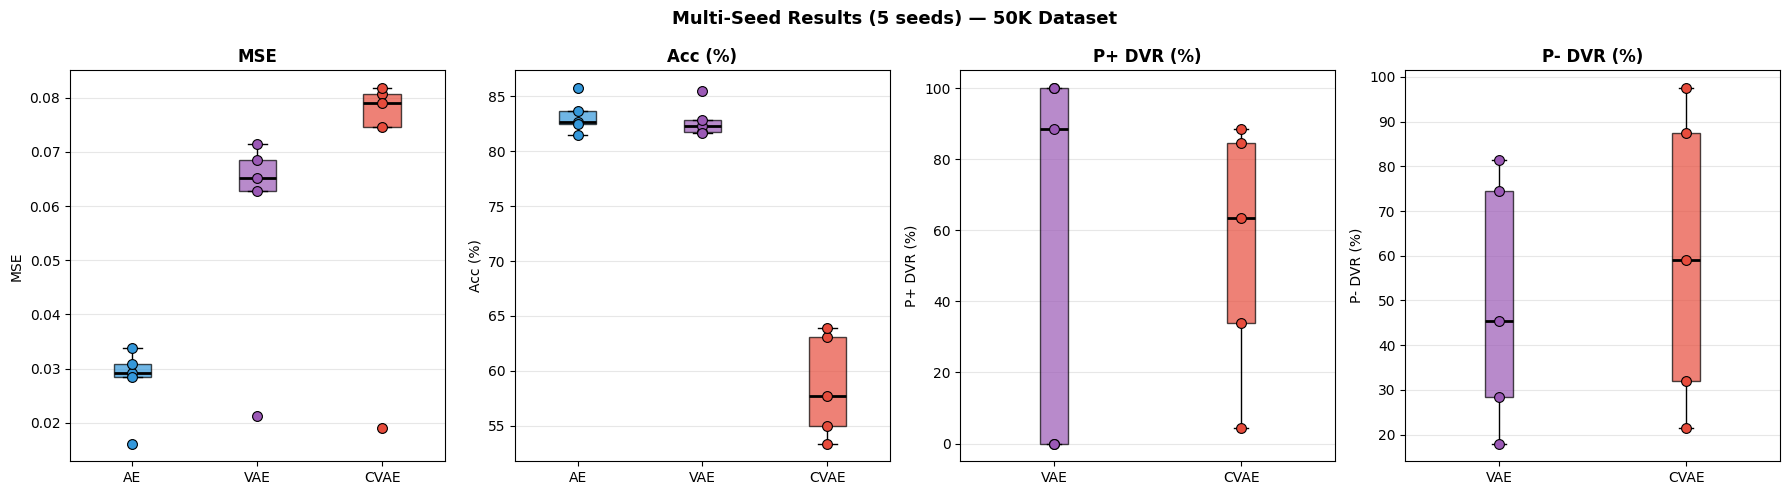
\includegraphics[width=1.0\textwidth]{figures/16_multiseed_boxplots.png}
    \caption{Multi-seed robustness results across reconstruction MSE, classification accuracy, $P^{+}$ DVR, and $P^{-}$ DVR.}
    \label{fig:multiseed_boxplots}
\end{figure}

Figure~\ref{fig:multiseed_boxplots} visually confirms the same trend as the tables. Reconstruction and classification results are comparatively more stable, especially for AE and VAE, while DVR has much larger variation across seeds.

\subsection{Robustness Summary}
\label{subsec:robustness_summary}

The multi-seed results should be interpreted across all metrics together. Reconstruction stability shows whether the model consistently learns the numerical objective-vector distribution. Classification stability shows whether the learned representation consistently separates $P^{+}$ and $P^{-}$. DVR stability shows whether generated samples consistently preserve the dominance relation.

The final robustness conclusion is summarized as follows:
\begin{compactitem}
    \item AE reconstruction stability: AE is the most stable reconstruction model, with the lowest mean MSE and lowest MSE standard deviation.
    \item VAE reconstruction and generation stability: VAE has stable classification performance close to AE, but its DVR is highly variable, especially for generated $P^{+}$ samples.
    \item CVAE class-controlled generation stability: CVAE enables class-conditioned generation, but it has weaker and less stable classification performance than AE and VAE.
    \item DVR stability across seeds: DVR is unstable for both VAE and CVAE, showing that dominance-preserving generation remains sensitive to random seed and latent sampling behavior.
\end{compactitem}

Since DVR variance remains high, the experiment supports the conclusion that dominance-preserving generation requires stronger constraint-aware learning mechanisms.